\chapter{Background}
\index{Background%
@\emph{Background}}%

When the Web was first created by Tim Berners-Lee in 1989, web pages were largely envisioned as static \textit{documents} with a single author or a small group of coordinating authors. 
The idea of composing a complex web application out of simple components like snapping together Lego blocks seemed like a distant dream at best.
Until recently, web authors were limited to using the predefined HTML elements or `tags' that were listed in the W3C standard and understood by browser programs, such as \tcode{<title>} and \tcode{<video>}. 
Creating your own \textit{sui generis} HTML elements with unique behaviors seemed beyond the capabilities of the web browsers of the day like Mosaic and Netscape Navigator.

As of early 2015, `modern' web apps are typically written with a Javascript framework that provides a cohesive set of structures, design patterns and practices designed to facilitate composing web applications, large or small, from a number of sub-components.
Angular, Meteor, and Backbone are three such frameworks.
The difference between a `framework' and a library is somewhat arbitrary, but typically frameworks are more comprehensive than narrowly focused utility libraries.
Yet all frameworks must exist within the confines of the programming model provided by the browser and the Document Object Model (DOM). 
In this model, the entire web page or app belongs to a single `document', constituent parts are not encapsulated or isolated from each other, and authors are limited to working with the predefined HTML tags.
These issues make it difficult to create and share generic, reusable \textit{web components} 
--- in the abstract sense --- 
among different users who may not use the same frameworks or follow the same set of assumptions and conventions.

\section{Current challenges in web authoring}
To illustrate how these problems affect the ability of authors to share and reuse code, let's look at an example from the popular Twitter Bootstrap library [CITE].
Twitter Bootstrap is a collection of Cascading Style Sheet (CSS) rules and Javascript widgets or components designed to allow web authors to quickly ``bootstrap'' an attractive, consistent look-and-feel onto a web page.
Bootstrap provides pre-styled User Interface (UI) widgets such as menus, buttons, panels, `dropdown' selectors, alerts, dialogs, and so on, to be used as building blocks to construct web sites or applications.
Because Bootstrap must work within the confines of the DOM and the HTML5 standard, this necessarily exposes a great deal of Bootstrap's internals to its users.
For example, to add a Bootstrap site navigation bar to your page, you must essentially copy and paste a large block of HTML and then customize it to your needs as shown in figure~\ref{f:twbs1}.

% 
\begin{figure}[htb]
\centering
 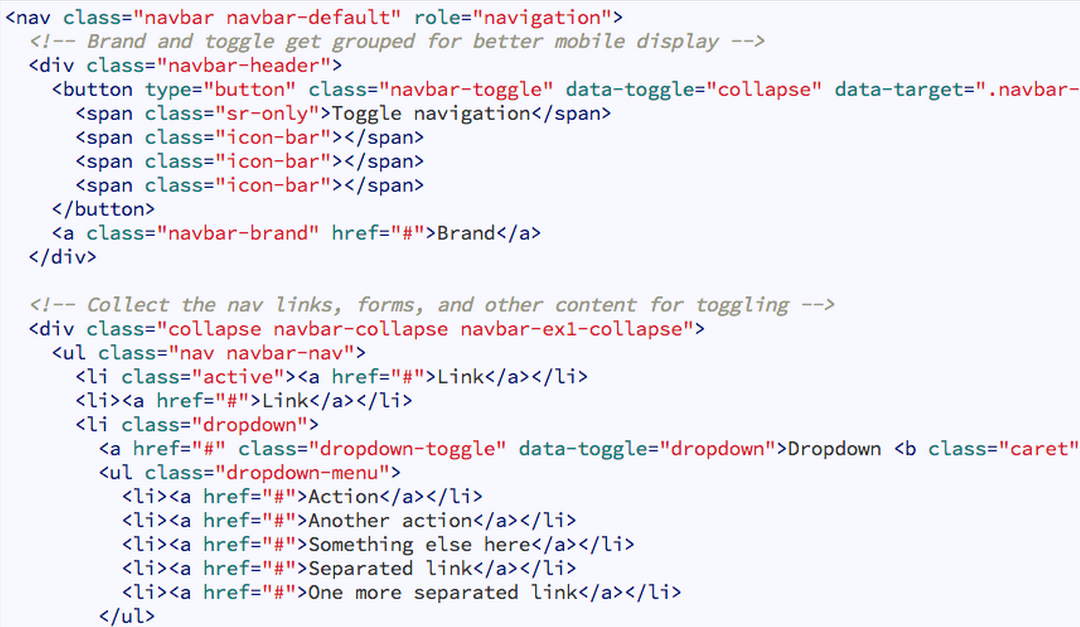
\includegraphics[width=6in]{images/bootstrap_navbar_html.png}
\caption{A partial example of Twitter Bootstrap navigation bar HTML.}
\label{f:twbs1}
\end{figure}
\index{commands!environments!figure}%

This forces Bootstrap's users to tightly couple the layout of their page with the internal structure required by Bootstrap's navigation bar widget. 
This coupling militates against Bootstrap significantly refactoring the internal structure of the navigation widget because that would require a large community of developers to update their applications accordingly.
In addition, because CSS rules normally apply across the entire page, the authors of Bootstrap must carefully select the scope and nomenclature of all rules to ensure minimal interference with other components and unintended effects. 
Even then, conflicts are inevitable when the entire page is treated as a single sandbox and you combine components from many different vendors. 

What if instead one could create and share a reusable chunk of functionality --- a web component -- that hid all of these tedious structural details and encapsulated its private, internal state? 
What if web authors could create their \textit{own} HTML elements?  
Using Bootstrap's navigation bar could be as simple as replacing the code in figure~\ref{f:twbs1} with a custom element like the one in figure~\ref{f:twbs2}.

% 
\begin{figure}[htb]
\centering
 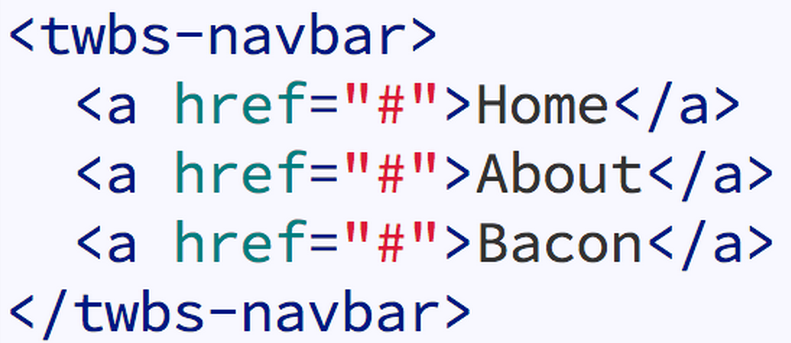
\includegraphics[width=3.5in]{images/bootstrap_navbar_wc.png}
\caption{Hypothetical Bootstrap nav bar custom element.}
\label{f:twbs2}
\end{figure}
\index{commands!environments!figure}%

\subsection{Encapsulation and composition}

The Web Components working group, consisting of software engineers from several major browser vendors, looked at this situation and found that, in practice, browsers already had a suitable model for encapsulating components that hide complexity behind well-defined interfaces.
That model was that one used internally by browsers to implement the newer HTML5 tags like the \textbf{\tcode{<video>}} element. 
The \tcode{<video>} element presents a simple interface (API) to HTML authors that hides the complexities of playing high definition video.
Internally, however, browsers implement \tcode{<video>} with a `shadow' or hidden document inside the object that contains the internal state. 
For example, an author can write:
\begin{lstlisting}[language=html]
	<video loop src=...> </video>
\end{lstlisting}
to cause the video to loop repeatedly.

This shadow Document Object Model (DOM) inside the \tcode{<video>} tag creates the user interface (UI) needed to control video playback such as volume controls, the timeline bar, and pause and play buttons.
These inner playback controls are themselves built out of HTML, CSS and JS but these details are not exposed to web authors who simply place a \tcode{<video>} element on their page. 
Figure~\ref{f:html5video} illustrates how this works. It shows the shadow (internal) DOM of a \tcode{<video>} element on a page with the \tcode{<div>} for the Play button highlighted.

% 
\begin{figure}[htb]
\centering
 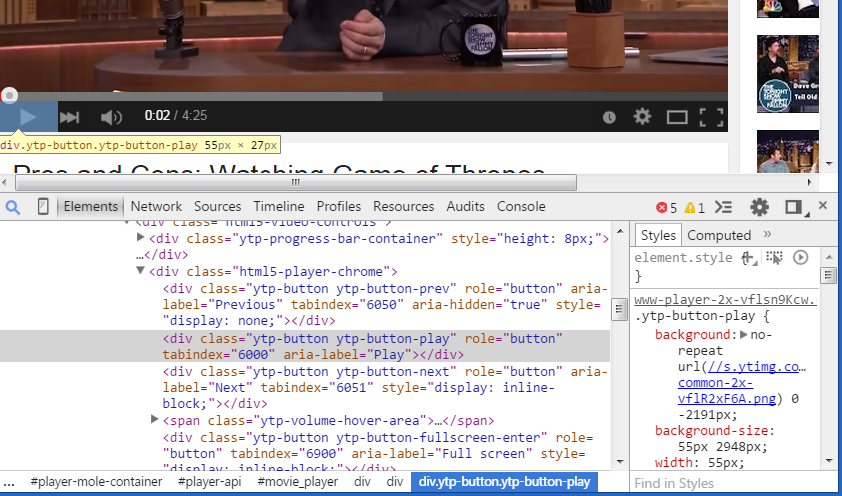
\includegraphics[width=5.5in]{images/html5_video_control.png}
\caption{Opera's shadow DOM for \tcode{<video>} highlighting the Play button}
\label{f:html5video}
\end{figure}
\index{commands!environments!figure}%

This example illustrates two design principles that are widely followed in other areas of software engineering [CITE]:
\begin{itemize}
\item The use of \textbf{encapsulation} and well defined interfaces, as the \tcode{<video>} element protects its private state and hides implementation complexity.
\item Prefer \textbf{composition} or \textit{has-a} relationships over inheritance or \textit{is-a} relationships when building modules. 
\end{itemize}
In the case of the interface for \tcode{<video>}, it's composed of simple block elements and scoped CSS roles and the Volume and Play controls aren't particularly special objects, just \texttt{<divs>} with CSS rules and click handlers.

The solution, therefore, to these coupling problems in web authoring is to expose these internal brower APIs for creating elements in a safe and portable fashion. 
This will allow web authors to create their own rich custom elements using standard portable APIs, encapsulate their internals, and enable easier sharing, composition and integration.
The question remains, which specific browser internals must be exposed and standardized in order to support Web Components?

\section{Web Components}

The Web Component initiative consists of two main technologies and two supporting features. 
Custom HTML Elements and Shadow DOM are the two key players while HTML Imports and Templates support these features.

\subsection{Custom HTML elements}
Never before have web authors been able to define their own custom HTML elements not found in the official list.
Actually, many authors and web frameworks have been doing exactly that for years, primarily for internal purposes where the custom elements are pre\-processed and compiled down to standard HTML.
The custom elements would not get sent to the end user's browser because the browser would not understand what to do with them.
However the possibility now exists to create custom elements in a standard way that will be supported by browsers. Technically, DOM has long supported creating custom-named elements, but it was not possible to do much interesting with them because they were treated like an ordinary \texttt{<span>}.

The primary restriction to avoid a name collision with future built-in HTML elements is that all custom elements must have a \texttt{-} character (dash) in their name, such as \texttt{<my-element>}.

To create a new Custom Element, first you register the element:

\begin{lstlisting}[language=Javascript]
 var MyElement = document.registerElement('my-element');
\end{lstlisting}

Then you place your new element on the page either declaratively in HTML:

\begin{lstlisting}[language=html]
 <my-element> hello, world! </my-element>
\end{lstlisting}

or imperatively with Javascript:

\begin{lstlisting}[language=Javascript]
 var MyElement = document.registerElement('my-element');
 // instantiate a new instance of the element
 var thisOne = new MyElement();      
 document.body.appendChild(thisOne); // add to the <body>
\end{lstlisting}


With a simple example like this the result does not look all that different from a \texttt{<span>}.
To do something more interesting with your custom element you will need to the other features of Web Components: Shadow DOM, templates and imports.

\subsection{Shadow DOM}
Shadow DOM encapsulates the internal structure of an element. 
As we have seen, browsers use Shadow DOM to encapsulate the private state of standard elements like \texttt{<video>} but now this capability is extended to custom-defined elements.

In general, Shadow DOM functions like a hidden, internal HTML document that describes the external appearance of the tag without exposing these details\footnote{
Shadow DOM should not be confused with the React framework's Virtual~DOM concept, which is closer in nature to Web Component Templates than Shadow DOM.
}. Typically a custom element definition has a template (more on those in a moment) which produces the shadow DOM necessary to render the element.
The actual contents of the shadow DOM are just ordinary elements.

Custom elements can wrap regular text, normal HTML elements, or other custom elements and then project that content into its own internal structure.
In the example in figure~\ref{f:twbs2} above, a simple \tcode{<twbs-navbar>} element consumes a set of three \tcode{<a>} (anchor or link) elements
but internally transforms that to something like the example in figure~\ref{f:twbs1}, 
projecting the set of links into the nav menu structure with appropriate wrappers.

Inside a custom element's template you use the \verb|<content>| tag to indicate the spot where the consumed (wrapped) content should be projected. 
This wrapped content is known as \textit{light DOM}, because it's given by the user and projected through into the shadow.
Together the shadow DOM and light DOM form the \textit{logical DOM} of a custom element.
It is also possible for elements to have multiple shadow DOM sub-trees. 
This is used particularly for emulating object-oriented inheritance.

In languages like C\# and Java, encapsulation often implies guarantees made by the language about the accessibility of object fields.
But in the case of Web Components, Shadow DOM is not completely and utterly isolated from the containing page.
It is possible to ``reach inside'' and break encapsulation to at least some degree, 
but the point is that this must be an intentional act by the developer and not an unexpected side-effect.

\subsection{HTML Imports}
One significant problem faced by web developers is that prior to Web Components, HTML lacked a mechanism to bring in a snippet of HTML or Javascript from an external location and insert it into the current document, similar to an \tcode{\#include} directive in the C language. 
Javascript could always be loaded with a \tcode{<script>} tag, but this did not ensure that resources were loaded exactly once, a process known as \textit{de-duping}.
If a component was used in two different spots on the page, it might need to use the same external Javascript resource but that file would be requested from the server twice, degrading application performance.

In order to fix these problems the HTML Imports standard allows for bringing in snippets of HTML, CSS or Javascript into the current document in a way that ensures automatic de-duping of repeated requests.
The one major caveat there is that de-duping only happens if the resources are named in exactly the same fashion in both cases.
More on that problem later (TODO: section).

\subsection{Templates}
Inert pieces of DOM that can be instantiated
Data-bound templates

\subsection{Related technologies}

Mutation Observers

CSS Flexbox

CSS Grid



\section{Literature Review}
\subsection{Popular Javascript frameworks}
\subsection{Google Polymer framework}

\section{Speakur}
\subsection{Origin}
\subsection{Motivations}

